\section{Transformación de modelo \gls{ecore} a modelo genmodel. Generación de proyectos editor Java a partir de modelos \gls{ecore}}

Los modelos \gls{ecore} proporcionan de forma abstracta una representación de meta-datos.
Para nuestro proyecto, necesitamos ser capaces de leer desde un programa todos estos datos desde un lenguaje de programación.

Esta transformación nos generará clases java a partir del formato \gls{ecore}, con el ahorro de tiempo considerable que esto supone. Clases observables según el método \gls{ecore}, y ampliables mediante interfaces y clases abstractas.

Esta transformación es personalizable en muchos aspectos, destacando a nivel de paquete y clase; ver figura 
\ref{fig:modelo_genmodel_paquete} donde podemos especificar que tipo de generación, paquete destino, nombres... utilizaremos para la transformación, y también a nivel de atributo de cada una de las propiedades 
, ver figura \ref{fig:modelo_genmodel_atributo} , donde podremos especificar con mucho detalle la generación de código, por ejemplo, indicando si el atributo utilizará las posibilidades de \gls{ecore} de observar cambios en el modelo en \gls{runtime}, especificar si la propiedad tendrá un icono en el editor \gls{ecore}, como será representado, por resumir, todas las propiedades necesarias para las cuatro generaciones de código base que proporciona.


\begin{figure}[p]
	\centering
    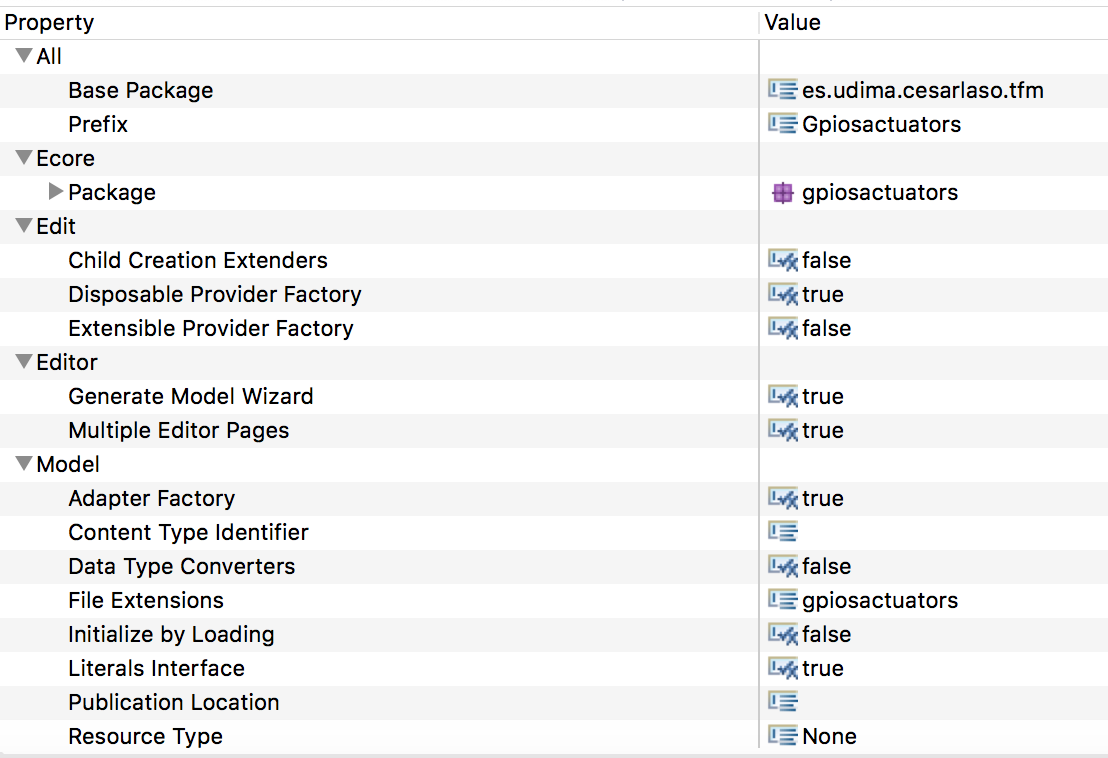
\includegraphics[scale=0.4]{images/emf_capturas/genmodel_paquete}
    \sourcepropia{}
    \caption{Especificación de propiedades del paquete y clases en su conversión a Java}
    \label{fig:modelo_genmodel_paquete}
\end{figure}

\begin{figure}[p]
	\centering
    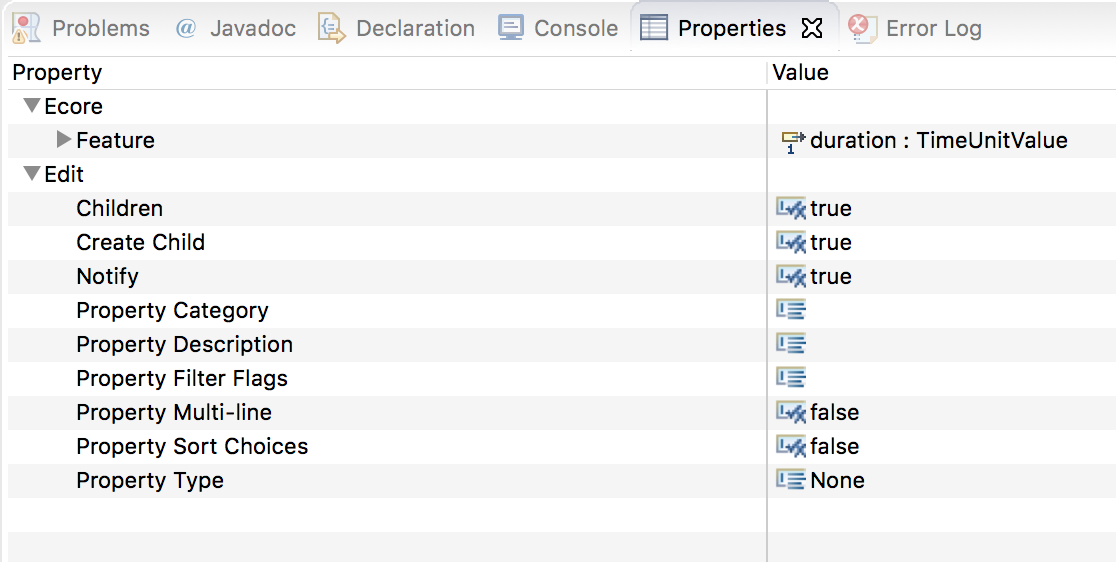
\includegraphics[scale=0.4]{images/emf_capturas/genmodel_atributo}
    \sourcepropia{}
    \caption{Genmodel - Especificación de propiedades del atributo de clase en su conversión a Java}
    \label{fig:modelo_genmodel_atributo}
\end{figure}


\gls{emf} proporciona una transformación de \gls{ecore} a archivos genmodel, la cual generará cuatro aspectos resultado en formato Java:

\begin{itemize}
    \item Código del modelo.
    \item Edición del modelo.
    \item Editor del modelo.
    \item Test unitarios.
\end{itemize}

\subsection{Código del modelo}

Primera transformación, base para todas las transformaciones posteriores. Nuestros metamodelos en formato \gls{ecore} han de ser transformados al lenguaje de programación Java para que podamos interactuar con ellos.

Esta transformación nos proporciona no solo código de las propiedades especificadas, sino que además nos proporciona código estático y tipado de los \gls{metadatos} de estas propiedades, lo que nos evita tener que inspeccionar en \gls{runtime} mediante \gls{reflection} estos elementos.

Otra generación muy interesante es que las clases generadas son interfaces java, con lo que tendremos posteriormente todas las posibilidades para aumentar su funcionalidad.

Debido a esta peculiaridad, esta generación de código nos proporciona clases base ya implementadas con la funcionalidad, así como factorías para construir estas clases.

Una vez generado el código, tendremos tres paquetes resultado en nuestro proyecto:

\begin{itemize}

\item Modelo. Interfaces con getters/setter del propio modelo. Ver ejemplo generado en figura \ref{fig:modelo_genmodel_gen_interface}.

\item Interface de la factoría. Utilizaremos para crear instancias. El nombre de la factoría, con la configuración por defecto será: ModeloFactory.eINSTANCE. Ver ejemplo generado en figura \ref{fig:modelo_genmodel_gen_factoria}. 

\item Interface del paquete de clase. Con información relevante con los datos transformados, con nombres de constantes, de forma fuertemente tipada, así como los métodos para acceder a esta información. Ver ejemplo generado en figura \ref{fig:modelo_genmodel_gen_paquete}.

\item Implementaciones tanto de los modelos como de las factorías. Ver ejemplo generado en las figuras \ref{fig:modelo_genmodel_impl_clase} y  \ref{fig:modelo_genmodel_impl_factoria}. Estas clases heredarán de sus interfaces base generadas y a su vez, de clases abstractas \gls{ecore}, con toda la funcionalidad añadida que aporta el propio framework, y diposible de forma tipada, sin necesidad.

\end{itemize}


\begin{figure}
	\centering
	
	\lstinputlisting[language=Java]{ejemplos/genmodel_gen_interface.java}
    
    \sourcepropia{}
    \caption{Fragmento de código con la interfaz en lenguaje Java generada a partir de modelo \gls{ecore} Pin}
    \label{fig:modelo_genmodel_gen_interface}
\end{figure}
\begin{figure}
	\centering
	
	\lstinputlisting[language=Java]{ejemplos/genmodel_gen_factoria.java}
	
    \sourcepropia{}
    \caption{Interfaz de la factoría Java generada a partir de modelo \gls{ecore}. Con esta factoria instanciaremos objetos}
    \label{fig:modelo_genmodel_gen_factoria}
\end{figure}
\begin{figure}
	\centering
	\lstinputlisting[language=Java]{ejemplos/genmodel_gen_paquete.java}
	
    
    \sourcepropia{}
    \caption{Propiedades del paquete con metadatos generados a partir de \gls{ecore}}
    \label{fig:modelo_genmodel_gen_paquete}
\end{figure}



\begin{figure}
	\centering
	\lstinputlisting[language=Java]{ejemplos/genmodel_impl_clase.java}
    \sourcepropia{}
    \caption{Resultado de la implementación de un interfaz generado por \gls{ecore}}
    \label{fig:modelo_genmodel_impl_clase}
\end{figure}

\begin{figure}
	\centering
	\lstinputlisting[language=Java]{ejemplos/genmodel_impl_factoria.java}
    
    \sourcepropia{}
    \caption{Resultado de la implementación del interfaz de una factoría \gls{ecore}}
    \label{fig:modelo_genmodel_impl_factoria}
\end{figure}



\subsection{Edición del modelo}

La generación de esta transformación \cite{emf_edit} da como resultado un proyecto adicional con el mismo nombre que nuestro proyecto más la extensión .edit.\newline
Este proyecto adicional, proporciona la base para el proyecto \textit{Edit}, proporcionando toda la funcionalidad necesaria basada en el propio \gls{ide} eclipse como editor.

En su parte de edición, proporciona soporte para la modificación de las propiedades de los modelos y la visualización estos mediante modelos EMF mediante el visor  \textcite{jface}.

Incluye un \gls{framework} de comandos para la construcción de editores, dando soporte automático a operaciones complejas como deshacer y rehacer.

Incluye un generador de código capaz de generar todo lo necesario para construir un \gls{plugin} editor, necesario para la siguiente transformación necesaria \textit{Editor del modelo}.

Todo este código puede ser personalizado, tanto en la primera transformación de la generación de este código, como en la posterior transformación, de este código que a su vez generará código para el editor de modelo. La ventaja y a su vez desventaja del código generado en compilación, es su validación y verificación. El código generado es fuertemente tipado, con lo que no podemos esperar errores en ejecución sobre objetos con tipos incorrectos o no construidos adecuadamente, ya que podemos añadir reglas \gls{ocl} \cite{ocl} en la validación de los modelos.

Se puede ver un ejemplo del proyecto generado en la figura \ref{fig:modelo_genmodel_edit} .

\begin{figure}
	\centering
    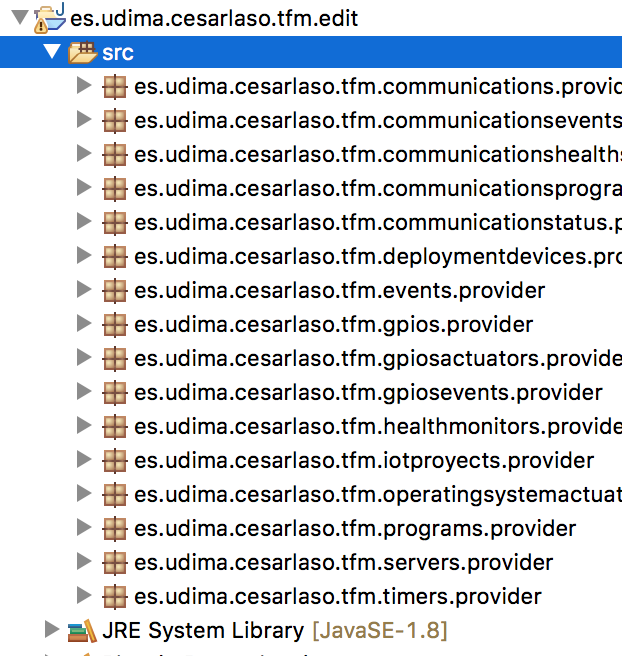
\includegraphics[scale=0.4]{images/emf_capturas/genmodel_edit}
    \sourcepropia{}
    \caption{Proyecto genmodel Edit, visualización de paquetes}
    \label{fig:modelo_genmodel_edit}
\end{figure}



\subsection{Editor del modelo}

Este proyecto es generado a partir de la información obtenida de las dos primeras transformaciones, primero transformando los modelos \gls{ecore} a código java mediante genmodel y posteriormente con las herramientas internas proporcionadas por Edit, a su vez obtenidas estas de los modelos \gls{ecore} transformados.

Este proyecto proporciona la capa de presentación para la edición de modelos de forma gráfica en el \gls{ide} eclipse.

Para ello, nos proporciona las siguientes herramientas:
\begin{itemize}
    \item \Gls{wizard} para la creación de proyectos basados en nuestros objetos \gls{ecore}.
    \item Editor gráfico de estos objetos generados.
\end{itemize}

La estructura de código generada, como podemos ver en la figura \ref{fig:modelo_genmodel_editor}, al igual que el anterior proyecto \textit{Edit}, sigue el mismo esquema, en este caso, nombre del proyecto más \textit{Editor}

\begin{figure}
	\centering
    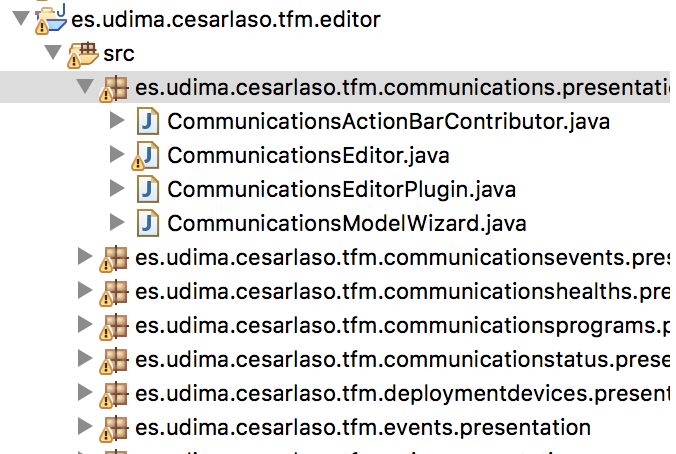
\includegraphics[scale=0.4]{images/emf_capturas/genmodel_editor}
    \sourcepropia{}
    \caption{Proyecto genmodel Editor, visualización de paquetes}
    \label{fig:modelo_genmodel_editor}
\end{figure}


El código generado, igualmente modificable, respeta entre código generado y código propio; tal como vemos en la  figura \ref{fig:modelo_genmodel_editor_codigo}, podemos observar el añadido de etiquetas \textit{generated} y como comentario html, con la etiqueta \texit{begin-user-doc} , la documentación si existiera que escribimos en el modelo \gls{ecore}.

\begin{figure}
	\centering
	
	\lstinputlisting[language=Java]{ejemplos/genmodel_editor_codigo.java}
    \sourcepropia{}
    \caption{Proyecto genmodel Editor, código generado}
    \label{fig:modelo_genmodel_editor_codigo}
\end{figure}


\subsection{Test unitarios}

Este proyecto generado, ya el último de los generados por genmodel, es utilizado para realizar tests unitarios de nuestro código java generado.

La estructura de directorios, es al igual que los anteriores: nombre más tipo proyecto. En este caso, \texit{Tests}, tal como vemos en la figura  \ref{fig:modelo_genmodel_tests}.

\begin{figure}
	\centering
    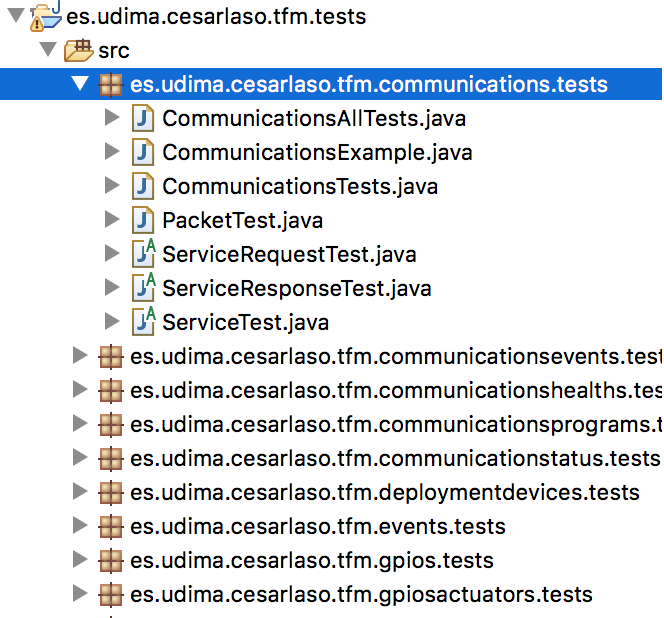
\includegraphics[scale=0.4]{images/emf_capturas/genmodel_tests}
    \sourcepropia{}
    \caption{Proyecto genmodel Tests, visualización de paquetes}
    \label{fig:modelo_genmodel_tests}
\end{figure}


El código generado es un esqueleto de tests unitarios que utilizan la librería \textit{standard} \cite{junit}, los cuales implementan una base con la que posteriormente trabajar, incluendo las dependencias necesarias para trabajar con junit y \gls{ecore}. Podemos ver un ejemplo de código generado en la figura \ref{fig:modelo_genmodel_tests_codigo}.

\begin{figure}
	\centering
	
	\lstinputlisting[language=Java]{ejemplos/genmodel_tests_codigo.java}
	
    \sourcepropia{}
    \caption{Proyecto genmodel Tests, código generado}
    \label{fig:modelo_genmodel_tests_codigo}
\end{figure}


\subsection{Pasos a realizar en la transformación}

Para cada meta modelo \gls{ecore} es necesaria la generación de su archivo generador de código java mediante su correspondiente archivo descriptor con extensión genmodel.

Los metamodelos EMF están formados por dos componentes, los propios metamodelos \gls{ecore} y los generadores. Este archivo descriptor nos ayuda a especificar como se ha de generar el código java respecto al modelo, pudiendo cambiar aspectos propios del lenguaje final de transformación (en el caso por defecto java).

A continuación, nos centramos en la plataforma de generación Java, y mostramos como realizar la generación de un \gls{metamodelo}, en este caso hemos elegido el \gls{metamodelo} GpioActuators. como ejemplo.

Los pasos a realizar para cada uno de los modelos \gls{ecore} son los siguientes:

\begin{enumerate}

\item Crear un nuevo archivo de tipo EMF generator model, según podemos ver en las figuras \ref{fig:modelo_genmodel_paso1} y \ref{fig:modelo_genmodel_paso2}. 
\item Escribir como nombre de archivo el mismo nombre que el archivo \gls{ecore} sin la extensión (figura  \ref{fig:modelo_genmodel_paso3}). Guardarlo en la carpeta destino model.

\item Seleccionar modelo origen. El generador permite seleccionar varios tipos de archivo fuente, tales como UML, RationalRose, o en este caso \gls{ecore} (figura  \ref{fig:modelo_genmodel_paso4}). Seleccionamos \gls{ecore} y seleccionamos desde el workspace el archivo GpioActuators.ecore (figura \ref{fig:modelo_genmodel_paso5}).

\item Seleccionamos el modelo principal GpioActuators y dejamos los modelos a los que se refiere como referencias ya que en los modelos referidos también vamos a generar código (figura \ref{fig:modelo_genmodel_paso6}). De esta forma podemos tener la generación de modelos separada.

\end{enumerate}

\begin{figure}
    \centering
    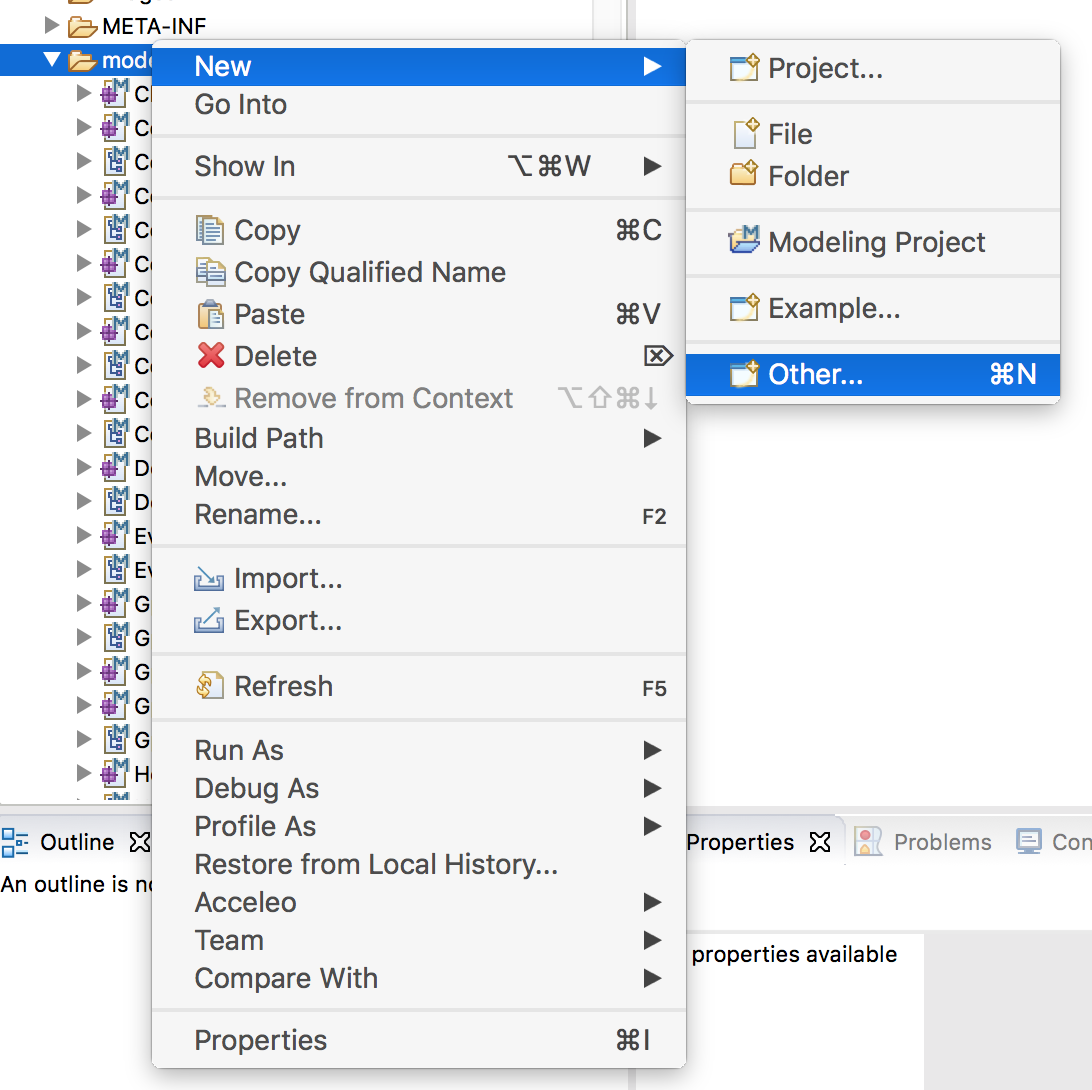
\includegraphics[scale=0.4]{images/emf_capturas/genmodel_1.png}
    \sourcepropia{}
    \caption[Creación de un archivo genmodel, paso 1]{Creación de un archivo genmodel. Si seleccionamos un archivo modelo, automáticamente en el \textit{wizard} tendremos la selección premarcada en el próximo paso.}
    \label{fig:modelo_genmodel_paso1}
\end{figure}

\begin{figure}
    \centering
    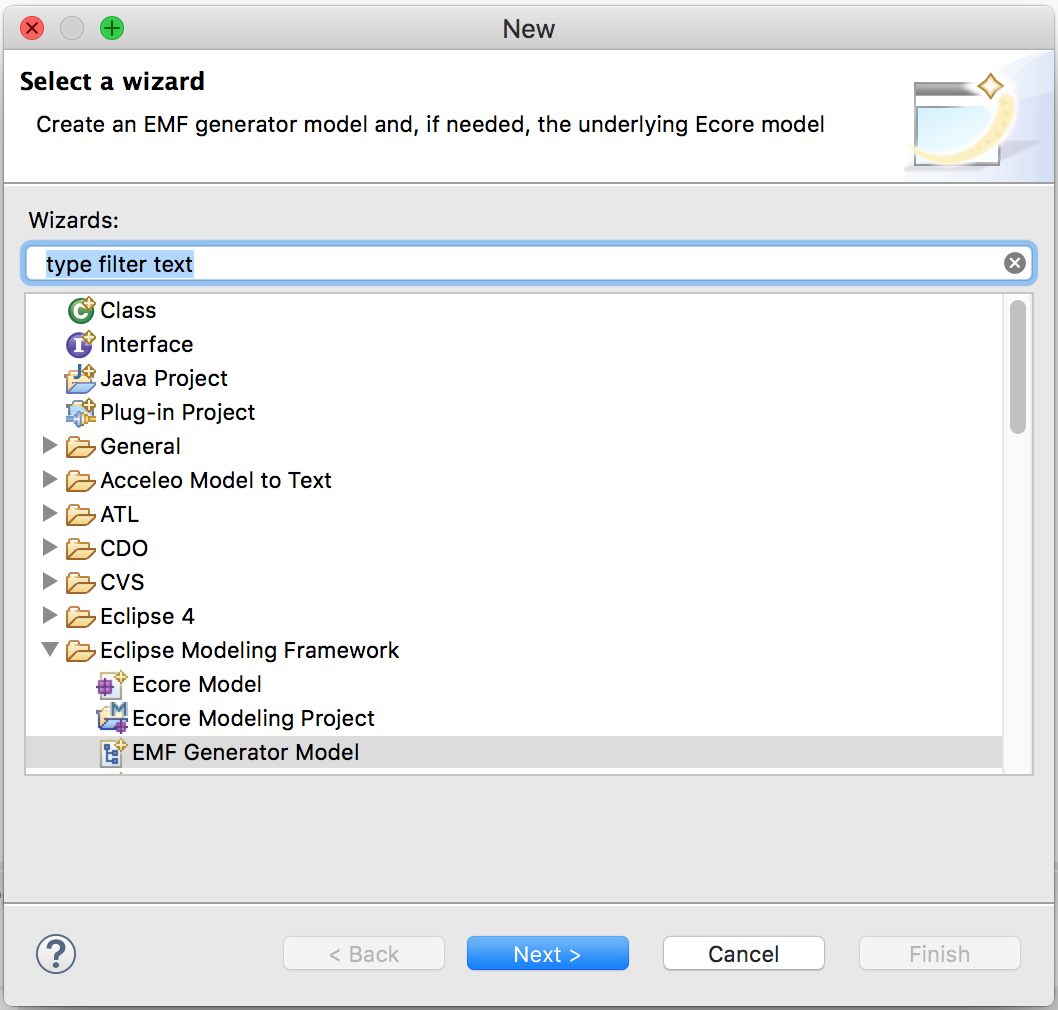
\includegraphics[scale=0.4]{images/emf_capturas/genmodel_2.png}
    \sourcepropia{}
    \caption[Creación de un archivo genmodel desde \gls{ecore}, paso 2]{EMF generator model permite la generación de proyectos de edición de código para java a partir de los modelos \gls{ecore}}
    \label{fig:modelo_genmodel_paso2}
\end{figure}

\begin{figure}
	\centering
    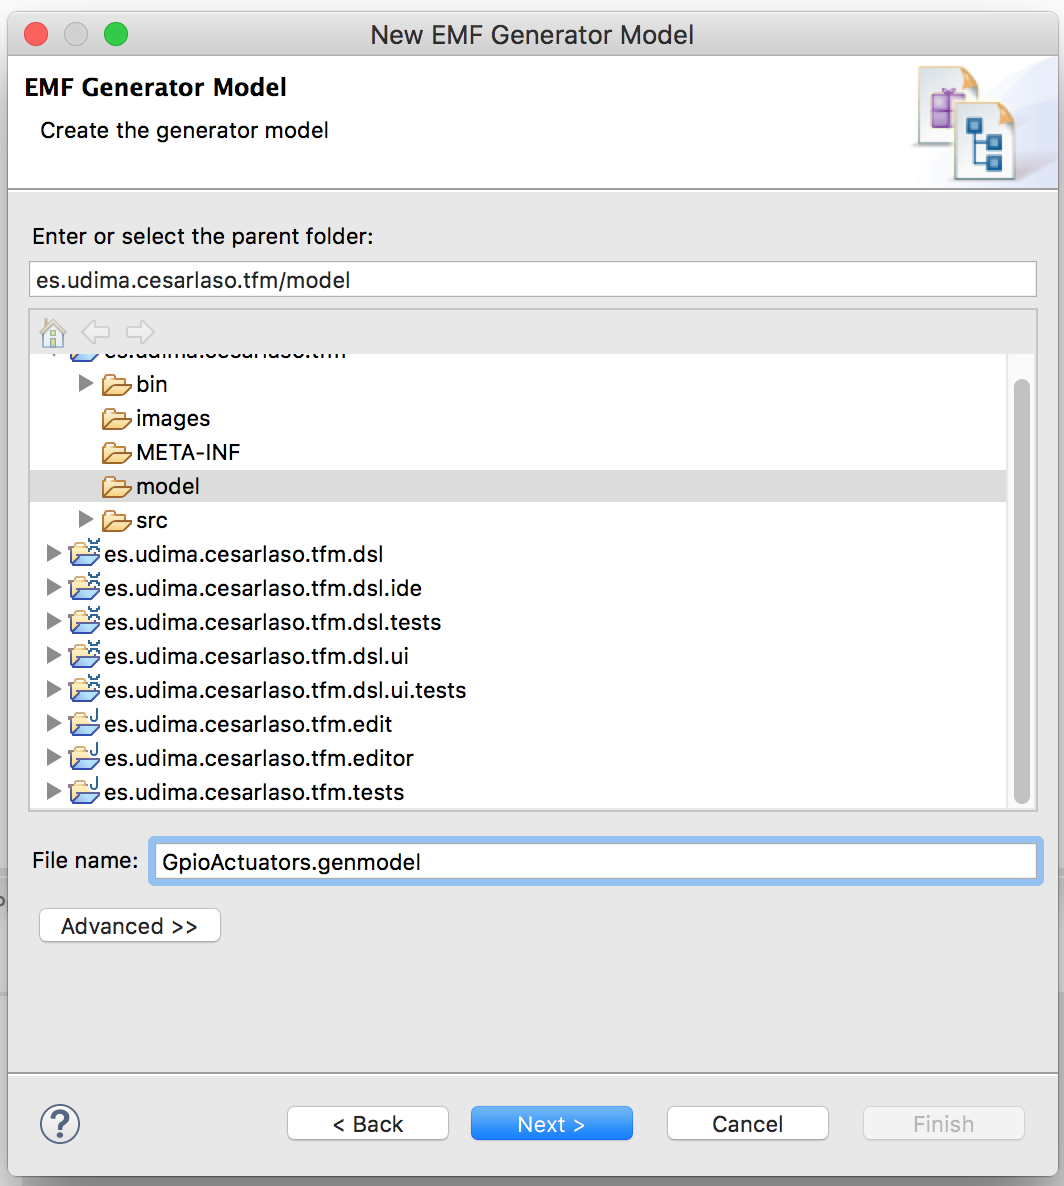
\includegraphics[scale=0.4]{images/emf_capturas/genmodel_3.png}
    \sourcepropia{}
    \caption[Creación de un archivo genmodel desde \gls{ecore}, paso 3]{Al generar el archivo genmodel se recomienda guardarlo en la misma ubicación que el archivo genmodel y con el mismo nombre que este.}
    \label{fig:modelo_genmodel_paso3}
\end{figure}
\begin{figure}
    \centering
    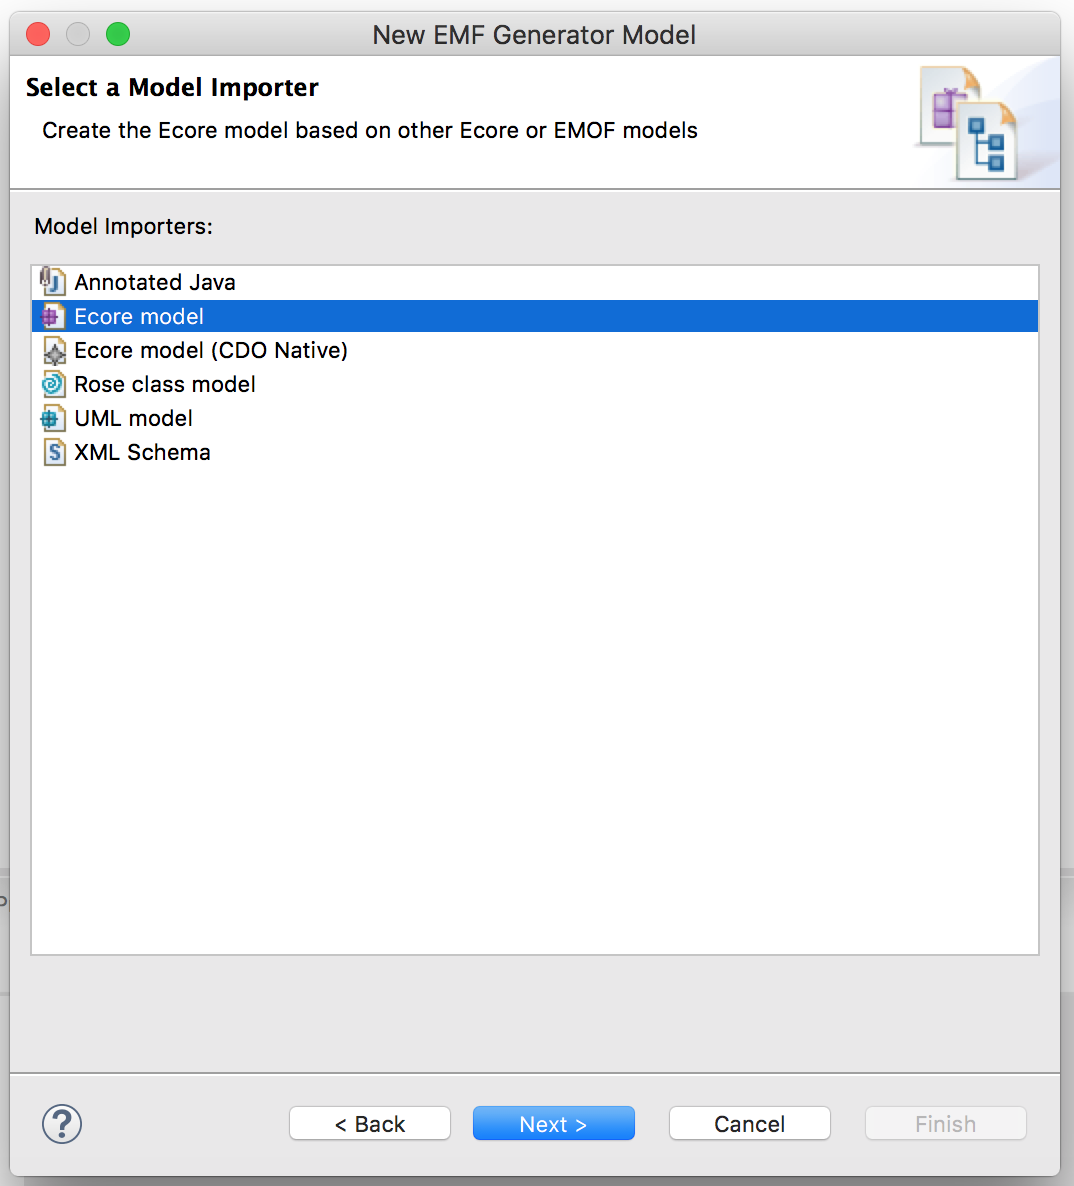
\includegraphics[scale=0.4]{images/emf_capturas/genmodel_4.png}
    \sourcepropia{}
    \caption[Genmodel desde otros tipos de modelado]{EMF genmodel permite la transformación de varios tipos de modelos, no solamente \gls{ecore}}
    \label{fig:modelo_genmodel_paso4}
\end{figure}
\begin{figure}
    \centering
    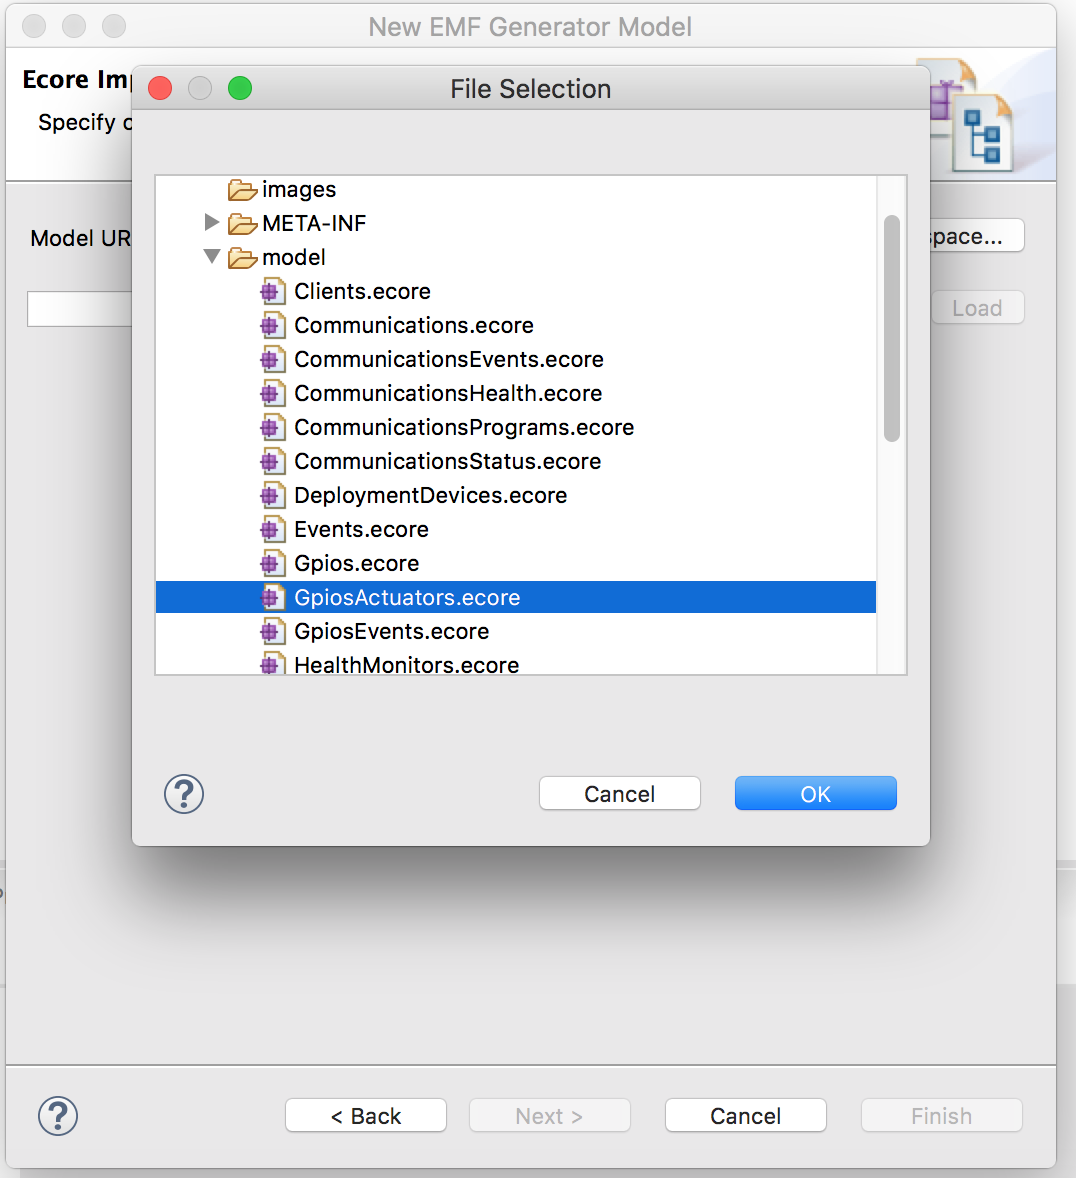
\includegraphics[scale=0.4]{images/emf_capturas/genmodel_5.png}
    \sourcepropia{}
    \caption[Genmodel ruta del proyecto]{EMF genmodel necesita conocer la ruta de los archivos modelo. En nuestro caso es recomendable utilizar la ruta relativa desde el workspace para mantener coherencia en el proyecto}
    \label{fig:modelo_genmodel_paso5}
\end{figure}
\begin{figure}
	\centering
    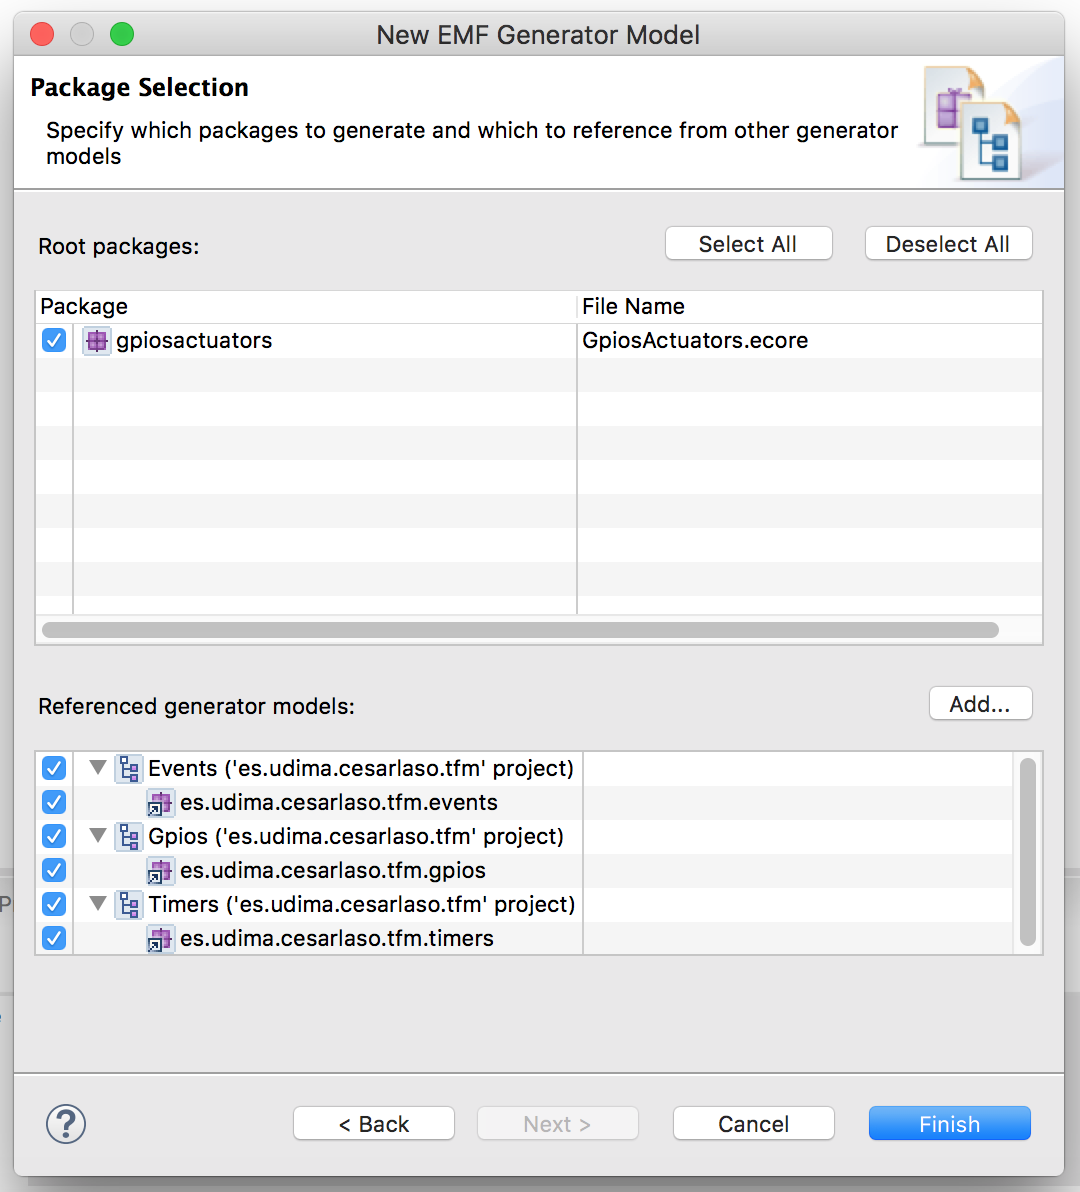
\includegraphics[scale=0.4]{images/emf_capturas/genmodel_6.png}
    \sourcepropia{}
    \caption[Genmodel selección de raíz y dependencias]{EMF genmodel necesita conocer cual es el modelo raíz y cuales sus dependencias. En caso de que el modelo dependa de otros archivos modelos, será necesario importarlos como referencia para que no genere el código por duplicado}
    \label{fig:modelo_genmodel_paso6}
\end{figure}



Una vez terminada la creación de los generadores de los modelos podemos modificar las propiedades sobre que se generará con el modelo, en nuestro caso solo modificaremos el nombre del paquete base ya que por defecto queda vacío, usaremos el mismo nombre de paquete que para el proyecto: \textit{es.udima.tfm.cesarlaso}.

Cada vez que modifiquemos el modelo \gls{ecore}, deberemos generar el código correspondiente mediante el genmodel. Es importante indicar que este proceso no se realiza automáticamente. Para ello es necesario mediante botón derecho o comando en menú, utilizar la opción de generar código: \textit{Generate All}. Existe la posibilidad de especificar que proyectos necesitamos generar (modelo, edit, editor o tests), como podemos observar en la figura  \ref{fig:modelo_genmodel_paso7}.

\begin{figure}
	\centering
    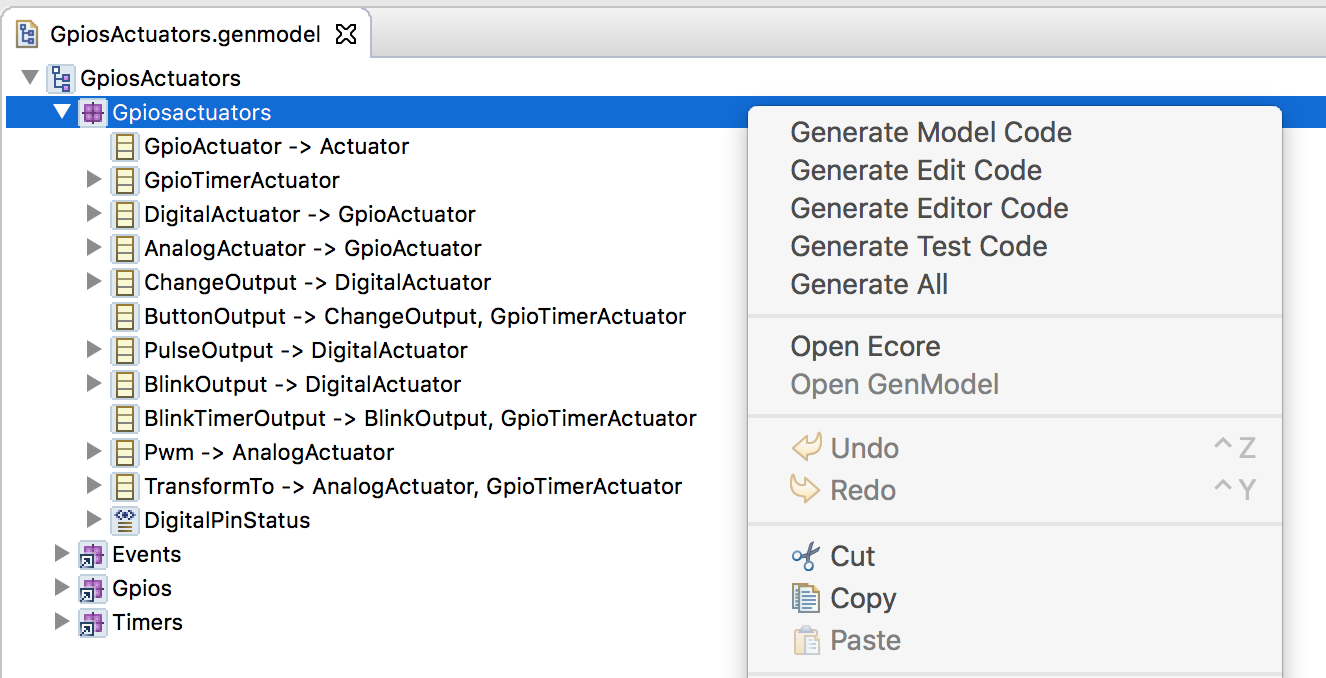
\includegraphics[scale=0.4]{images/emf_capturas/genmodel_7.png}
    \sourcepropia{}
    \caption[Genmodel selección de proyectos a generar]{Generación de código de proyecto desde genmodel. La generación permite seleccionar que proyecto que necesitamos generar. Incluye la posibilidad de generar todos a la vez.}
    \label{fig:modelo_genmodel_paso7}
\end{figure}


Una característica no resuelta en el generador de código de proyecto es que no es capaz de resolver inconsistencias de forma automática. Dependiendo del tipo de modificación que estemos realizando, cambio de tipo atributos, eliminar propiedades, será necesario eliminar todos los archivos generados por los generadores dentro de la carpeta \textit{src} del propio proyecto contenedor de los modelos. También deberemos eliminar los proyectos adicionales generados de \textit{edit, editor y test}. Dependiendo del tipo de modificación, como por ejemplo cambio del nombre del paquete, será necesario cambiar los archivos \textit{build.properties, plugin.xml y plugin.properties} , eliminando todas las referencia a modelos no existentes, hayan cambiado de nombre de paquete o de clase.

Una vez eliminados y realizadas las modificaciones correspondientes, procederemos a la generación de los archivos de proyecto java a partir de los modelos \gls{ecore}. Este proceso lo podemos realizar de forma granular para un modelo en concreto, seleccionando el archivo genmodel correspondiente y generando el código necesario tal como vimos en la figura \ref{fig:modelo_genmodel_paso5}.

A su vez contamos con un método de generación de todo el proyecto de una sola vez, lo que nos ahorra tiempo, mediante la combinación de teclado \textit{ALT+SHIFT+G}  podemos generar todo el código asociado a los modelos \gls{ecore} de una sola vez, tal como vemos en la figura \ref{fig:modelo_genmodel_paso8}. En el siguiente paso necesitaremos especificar qué tipos de proyectos generados necesitaremos (ver figura \ref{fig:modelo_genmodel_paso9}). Por defecto se seleccionarán todos.


\begin{figure}
    \centering
    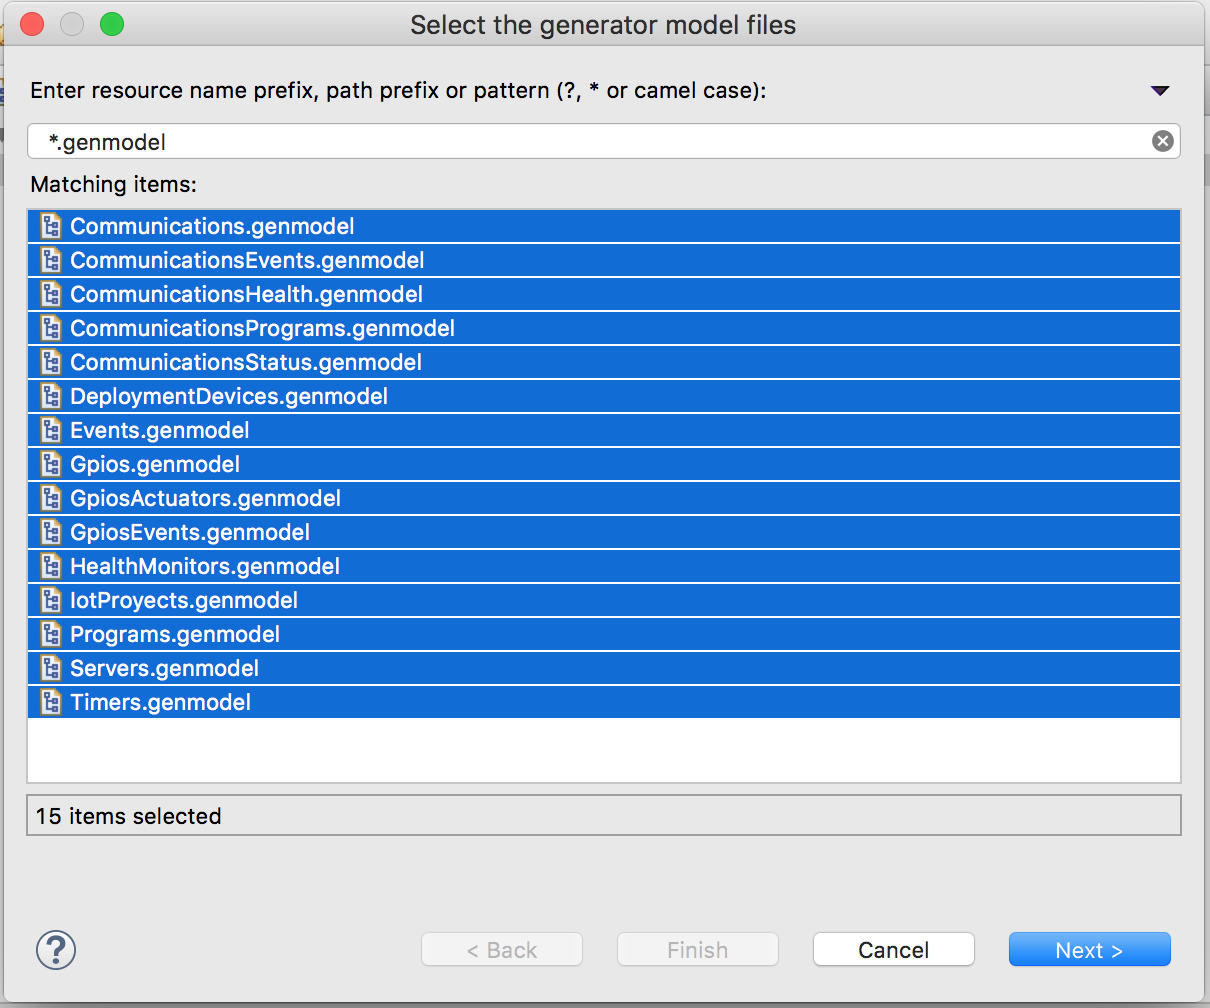
\includegraphics[scale=0.4]{images/emf_capturas/genmodel_8.png}
    \sourcepropia{}
    \caption[Genmodel generación de proyectos desde varios modelos simultáneamente]{EMF generatormodel permite la generación desde varios modelos de forma simultanea, pulsando \textit{ALT+SHIFT+G}. Permite seleccionar los modelos necesarios}
    \label{fig:modelo_genmodel_paso8}
\end{figure}

\begin{figure}
    \centering
    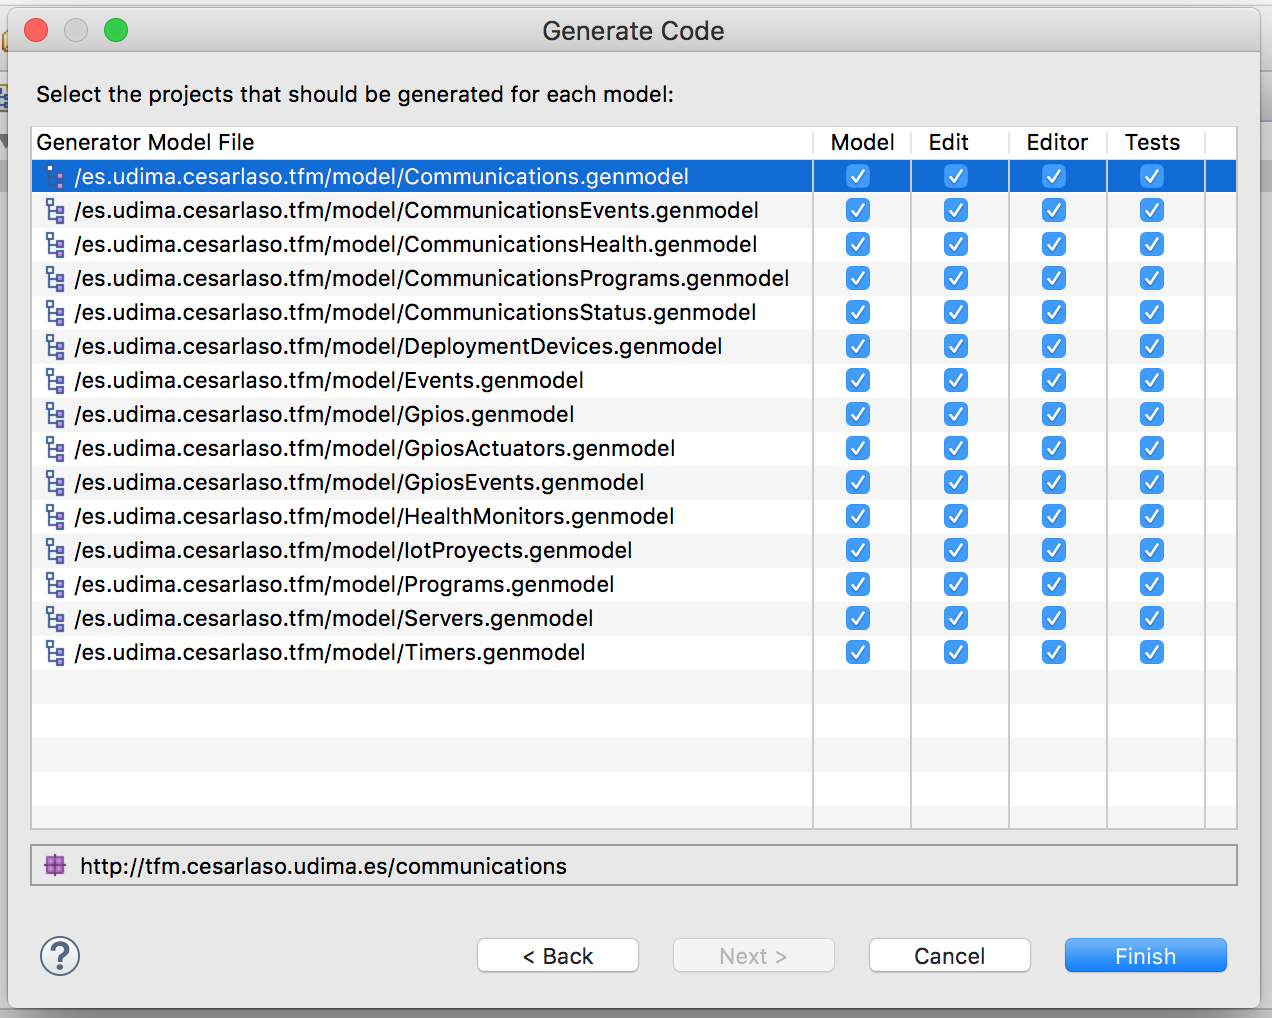
\includegraphics[scale=0.4]{images/emf_capturas/genmodel_9.png}
    \sourcepropia{}
    \caption[Genmodel selección de tipo de proyecto multiple]{EMF generatormodel en su vista de generación múltiple permite en una sola vista seleccionar el tipo de proyectos a generar para cada modelo \gls{ecore}. Permite seleccionar model,edit,editor,test}
    \label{fig:modelo_genmodel_paso9}
\end{figure}



\subsection{Generadores Ecore a genmodel para otros lenguajes}

Existen generadores a otros lenguajes como C++ mediante el proyecto \cite{emf4cpp_home} de la universidad de Murcia, podemos descargar el \cite{emf4cpp_code} código desde su propia web. Esta implementación actualmente incluye el parser de modelos desde C++ y generación de código a C++, el resto de funcionalidades tales como reflexión del propio \gls{metamodelo} aún no están listas.
Según el changelog, la última actualización es de 2010 por lo que podemos suponer que una vez terminada la cátedra se ha abandonado el proyecto.
